\documentclass{beamer}
\usepackage{clrscode}
\usepackage{graphicx}
\usepackage{booktabs}
\usepackage[most]{tcolorbox}
\usepackage{ragged2e}
\usepackage{amsmath, esint}
\usepackage[symbol]{footmisc}
\usepackage{tikz}
\usetikzlibrary{backgrounds, positioning, arrows, scopes, shapes, shapes.misc, shapes.multipart}
\tikzset{
    cross/.style={cross out, draw=black, minimum size=2*(#1-\pgflinewidth), inner sep=0pt, outer sep=0pt},
    cross/.default={10pt},
    split/.style={rectangle split, rectangle split parts=7, draw, inner sep=0ex, rectangle split horizontal, minimum size=4ex},
    textstyle/.style={text height=1.5ex, text depth=.25ex}
}

\usepackage{amsthm}
\usepackage{amstext}
\usepackage{amssymb}

\usepackage{minted}
\usepackage{xcolor}
\definecolor{LightGray}{gray}{0.975}

\renewcommand{\qed}{\\ \hfill $\blacksquare$}

%\usetheme{Warsaw}
\usefonttheme{serif}

\title[L6 DP Ex]{Introduction to Algorithms \\ Lecture 7: DP Exercises}
\author{Cormen, Leiserson, Rivest, and Stein. MIT Press. 2022.}
\date{\today}

\setbeamertemplate{navigation symbols}{}%remove navigation symbols

\defbeamertemplate*{footline}{shadow theme}{%
    \leavevmode%
    \hbox{
        \begin{beamercolorbox}[wd=.5\paperwidth,ht=2.5ex,dp=1.125ex,leftskip=.3cm plus1fil,rightskip=.3cm]{author in head/foot}%
            \usebeamerfont{author in head/foot} Introduction to Algorithms: \hfill \insertshorttitle
        \end{beamercolorbox}%
        \begin{beamercolorbox}[wd=.5\paperwidth,ht=2.5ex,dp=1.125ex,leftskip=.3cm,rightskip=.3cm plus1fil]{title in head/foot}%
            \usebeamerfont{title in head/foot} \hfill \insertframenumber\,/\,\inserttotalframenumber%
        \end{beamercolorbox}
    }%
    \vskip0pt%
}

\AtBeginSection[]{
    \begin{frame}<beamer>
    \frametitle{Plan}
    \tableofcontents[currentsection]
    \end{frame}
}

\newcommand{\toRight}[1]{
    \begin{FlushRight}
        {\small #1}
    \end{FlushRight}
}

\begin{document}

\frame{\titlepage}

\begin{frame}{Introduction to Algorithms}
    \centering
    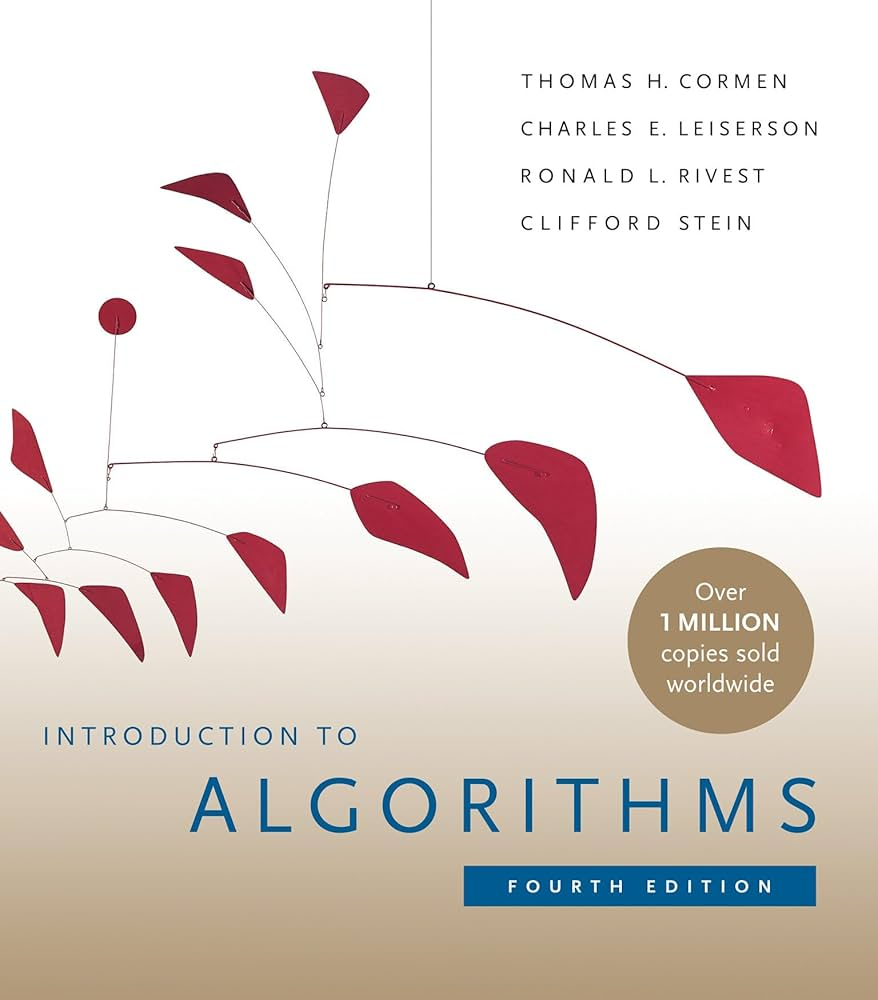
\includegraphics[width=0.45\textwidth]{figures/book_cover.jpg} \\
    \vspace{5mm}{
        \tiny
        Content has been extracted from \textit{Introduction to Algorithms}, Fourth Edition, by Cormen, Leiserson, Rivest, and Stein. MIT Press. 2022.\\
        Visit \url{https://mitpress.mit.edu/9780262046305/introduction-to-algorithms/}.
    }
\end{frame}

\section{Matrix-chain multiplication}

\begin{frame}{Matrix-chain multiplication}
    \textbf{Problem}: Given a sequence (chain) $\langle A_1, A_2, \ldots, A_n\rangle$ of $n$ matrices, compute the product $A_1 A_2 \cdots A_n$ using standard matrix multiplication (not Strassen's method) while minimizing the number of scalar multiplications.

    \begin{alertblock}{}
        How to parenthesize the product to minimize the number of scalar multiplications?
    \end{alertblock}
\end{frame}

\begin{frame}{Matrix-chain multiplication}
    \begin{itemize}
        \item Suppose multiplying matrices A and B: $C = A \cdot B$.
        \item The matrices must be compatible: number of columns of $A$ equals number of rows of $B$.
        \item If A is $p \times q$ and B is $q \times r$, then C is $p \times r$ and takes $pqr$ scalar multiplications.
    \end{itemize}
\end{frame}

\begin{frame}{Example}
    $A_1: 10 \times 100$, $A2: 100 \times 5$, $A3: 5 \times 50$. Compute $A_1 A_2 A_3$, which is $10 \times 50$.
    \begin{itemize}
        \item Try parenthesizing by $((A_1 A_2) A_3)$. First perform $10 \times 100 \times 5 = 5000$ multiplications, then perform $10 \times 5 \times 50 = 2500$, for a total of 7500.
        \item Try parenthesizing by $(A_1 (A_2 A_3))$. First perform $100 \times 5 \times 50 = 25,000$ multiplications, then perform $10 \times 100 \times 50 = 50,000$, for a total of 75,000.
        \item The first way is 10 times faster.
    \end{itemize}
\end{frame}


\begin{frame}{Input to the Problem}
    \begin{itemize}
        \item Let $A_i$ be $p_{i - 1} \times p_i$. The input is the sequence of dimensions $\langle p_0, p_1, p_2, \ldots , p_n \rangle$.
        \item \textbf{Note}: Not actually multiplying matrices. Just deciding an order with the lowest cost.
    \end{itemize}
\end{frame}

\begin{frame}{Counting the Number of Parenthesizations}
    \begin{itemize}
        \item Let $P(n)$ denote the number of ways to parenthesize a product of $n$ matrices. $P(1) = 1$.
        \item When $n \geq 2$, can split anywhere between $A_k$ and $A_{k + 1}$ for $k = 1, 2, \ldots, n - 1$. Then have to split the subproducts.
        \item Get
            \begin{equation*}
                \begin{align*}
                    P(n) =
                        \begin{cases}
                            1 & \text{ if } n = 1 \text{, } \\
                            \sum_{k = 1}^{n - 1} P(k)P(n - k) & \text{ if } n \geq 2 \text{.}
                        \end{cases}
                \end{align*}
            \end{equation*}
        \item The solution is $P(n) = \Omega \left( \frac{4^n}{n^{\frac{3}{2}}} \right)$. So brute force is a bad strategy.
    \end{itemize}
\end{frame}

\begin{frame}{Step 1: Structure of an optimal solution}
    \begin{itemize}
        \item Let $A_{i:j}$ be the matrix product $A_i A_{i+1} \cdots A_j$.
        \item If $i < j$, then must split between $A_k$ and $A_{k+1}$ for some $i \leq k < j \Rightarrow$  compute $A_{i:k}$ and $A_{k+1:j}$ and then multiply them together.
        \item Cost is
            \begin{equation*}
                \begin{align*}
                        & \text{ cost of computing } A_{i:k} \\
                    +   & \text{ cost of computing } A_{k+1:j} \\
                    +   & \text{ cost of multiplying them together.}
                \end{align*}
            \end{equation*}
    \end{itemize}
\end{frame}

\begin{frame}{Optimal substructure}
    \begin{itemize}
        \item Suppose that optimal parenthesization of $A_{i:j}$ splits between $A_k$ and $A_{k+1}$.
        \item Then the parenthesization of $A_{i:k}$ must be optimal.
        \item Otherwise, if there's a less costly way to parenthesize it, you'd use it and get a parenthesization of $A_{i:j}$ with a lower cost. Same for $A_{k+1:j}$.
        \item Therefore, to build an optimal solution to $A_{i:j}$:
            \begin{itemize}
                \item split it into how to optimally parenthesize $A_{i:k}$ and $A_{k+1:j}$,
                \item find optimal solutions to these subproblems,
                \item and then combine the optimal solutions.
            \end{itemize}
        \item Need to consider all possible splits.
    \end{itemize}
\end{frame}

\begin{frame}{Step 2: A recursive solution}
    \begin{itemize}
        \item Define the cost of an optimal solution recursively in terms of optimal subproblem solutions.
        \item Let $m[i, j]$ be the minimum number of scalar multiplications to compute $A_{i:j}$. For the full problem, want $m[1, n]$.
        \begin{itemize}
            \item If $i = j$, then just one matrix $ m[i, i] = 0$ for $i = 1, 2, \ldots, n$.
            \item If $i < j$, then suppose the optimal split is between $A_k$ and $A_{k+1}$, where $i \leq k < j$.
            \item Then $m[i, j] = m[i, k] + m[k+1, j] + p_{i-1} p_i p_j$.
        \end{itemize}
    \end{itemize}
\end{frame}

\begin{frame}{Step 2: A recursive solution}
    \begin{itemize}
        \item But that's assuming you know the value of $k$. Have to try all possible values and pick the best, so that
            \begin{equation*}
                \scriptsize
                \begin{align*}
                    m[i, j] =
                        \begin{cases}
                            0 & \text{ if } i = j \text{,} \\
                            min \{ m[i, k] + m[k+1, j] + p_{i-1} p_k p_j : i \leq k < j \} & \text{ if } i < j \text{.}
                        \end{cases}
                \end{align*}
            \end{equation*}
        \item That formula gives the cost of an optimal solution, but not how to construct it.
            \begin{itemize}
                \item Define $s[i, j]$ to be a value of $k$ to split $A_{i:j}$ in an optimal parenthesization.
                \item Then $s[i; j] = k$ such that $m[i, j] = m[i, k] + m[k+1, j] + p_{i-1} p_k p_j$.
            \end{itemize}
    \end{itemize}
\end{frame}

\begin{frame}{Step 3: Compute the optimal costs}
    \begin{itemize}
        \item Could implement a recursive algorithm based on the above equation for $m[i, j]$ but it would take exponential time.
        \item There are not all many subproblems:
            \begin{itemize}
                \item just one for each $i, j$ such that $1 \leq i \leq j \leq n$.
                \item there are ${n \choose 2} + n = \Theta (n^2)$ of them.
                \item thus, a recursive algorithm would solve the same subproblem over and over.
            \end{itemize}
        \item In other words, this problem has overlapping subproblems.
    \end{itemize}
\end{frame}

\begin{frame}{Step 3: Compute the optimal costs}
    \begin{itemize}
        \item Here is a tabular, bottom-up method to solve the problem.
        \item It solves subproblems in order of increasing chain length.
    \end{itemize}
    \centering
    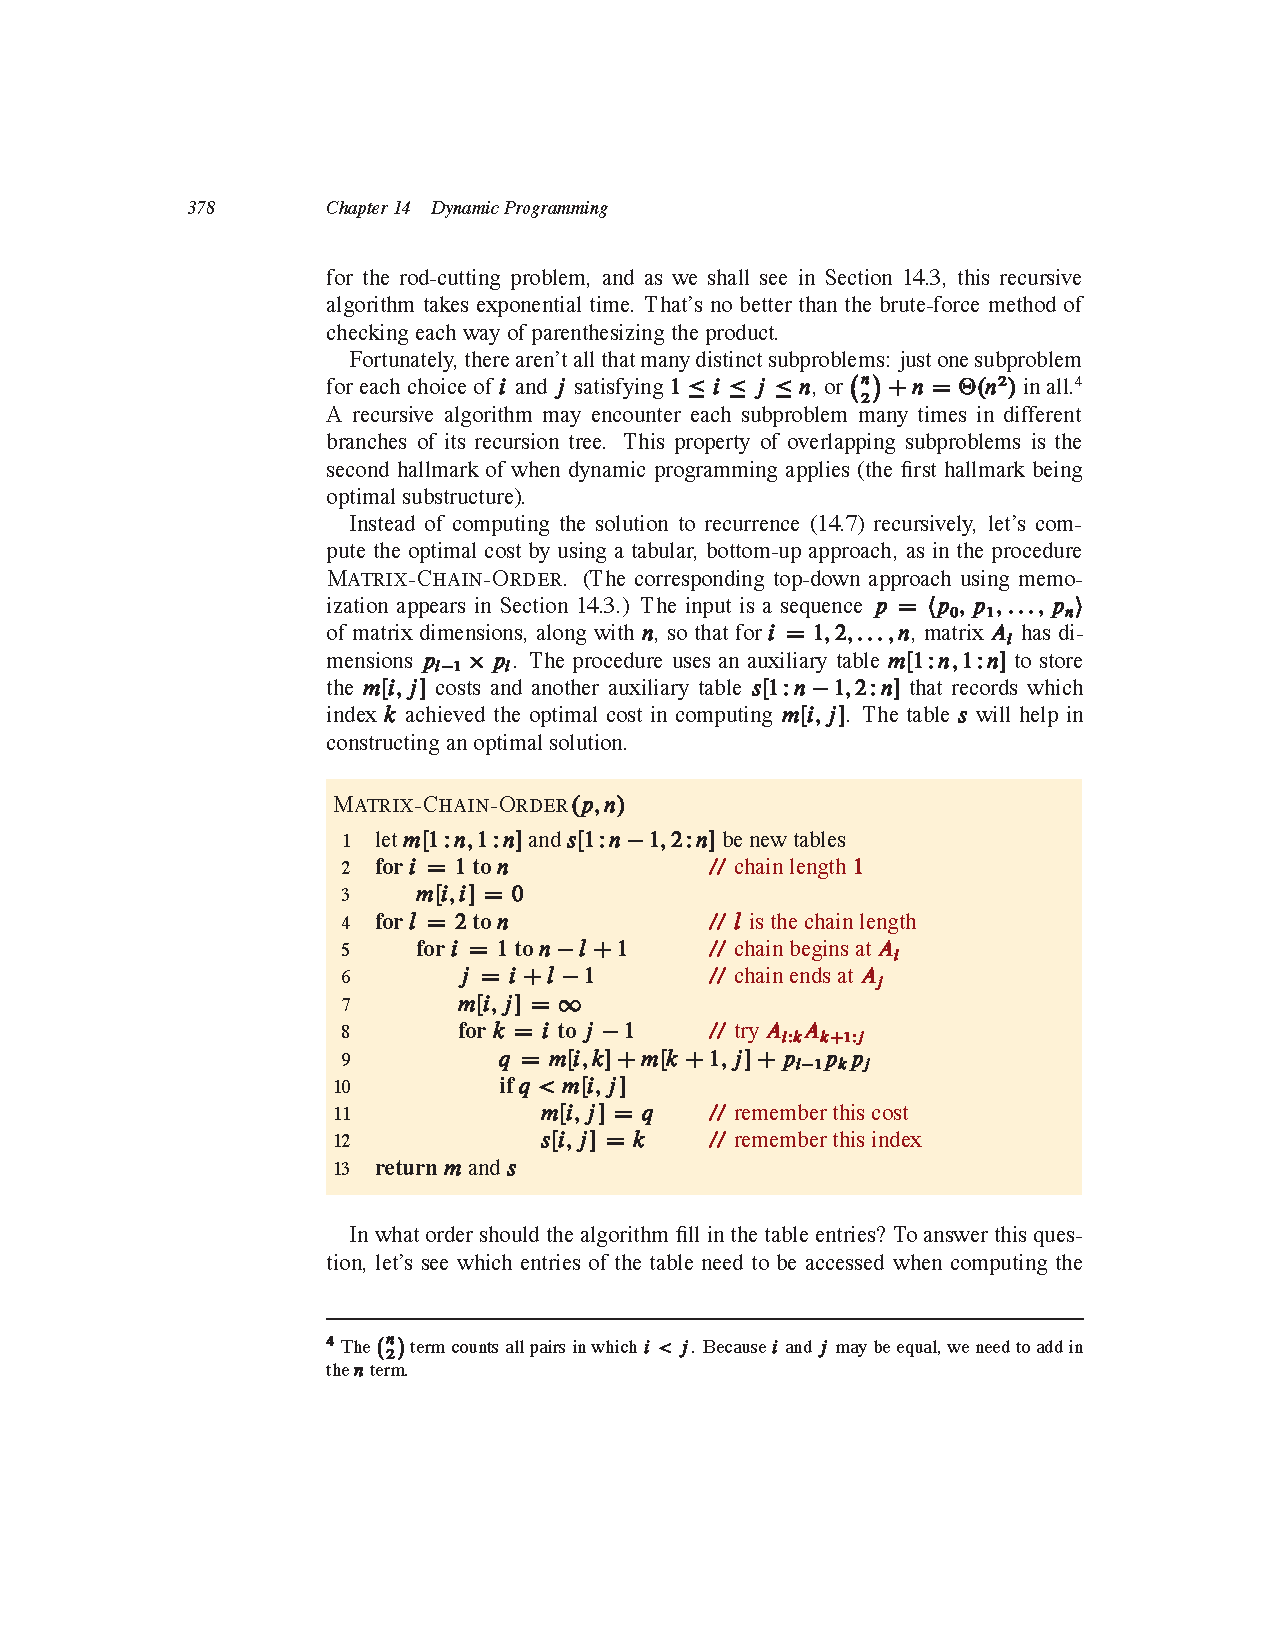
\includegraphics[width=\textwidth, trim={4cm 7.5cm 3cm 13cm}, clip]{figures/p378} \pause
    \textbf{Time}: $O(n^3)$, from triply nested loops. Also $\Omega (n^3) \Rightarrow \Theta (n^3)$.
\end{frame}

\begin{frame}{Step 4: Construct an optimal solution}
    \begin{itemize}
        \item With the $s$ table filled in, recursively print an optimal solution.
        \item Initial call is \textsc{Print-Optimal-Parens}$(s, 1, n)$.
    \end{itemize}
    \centering
    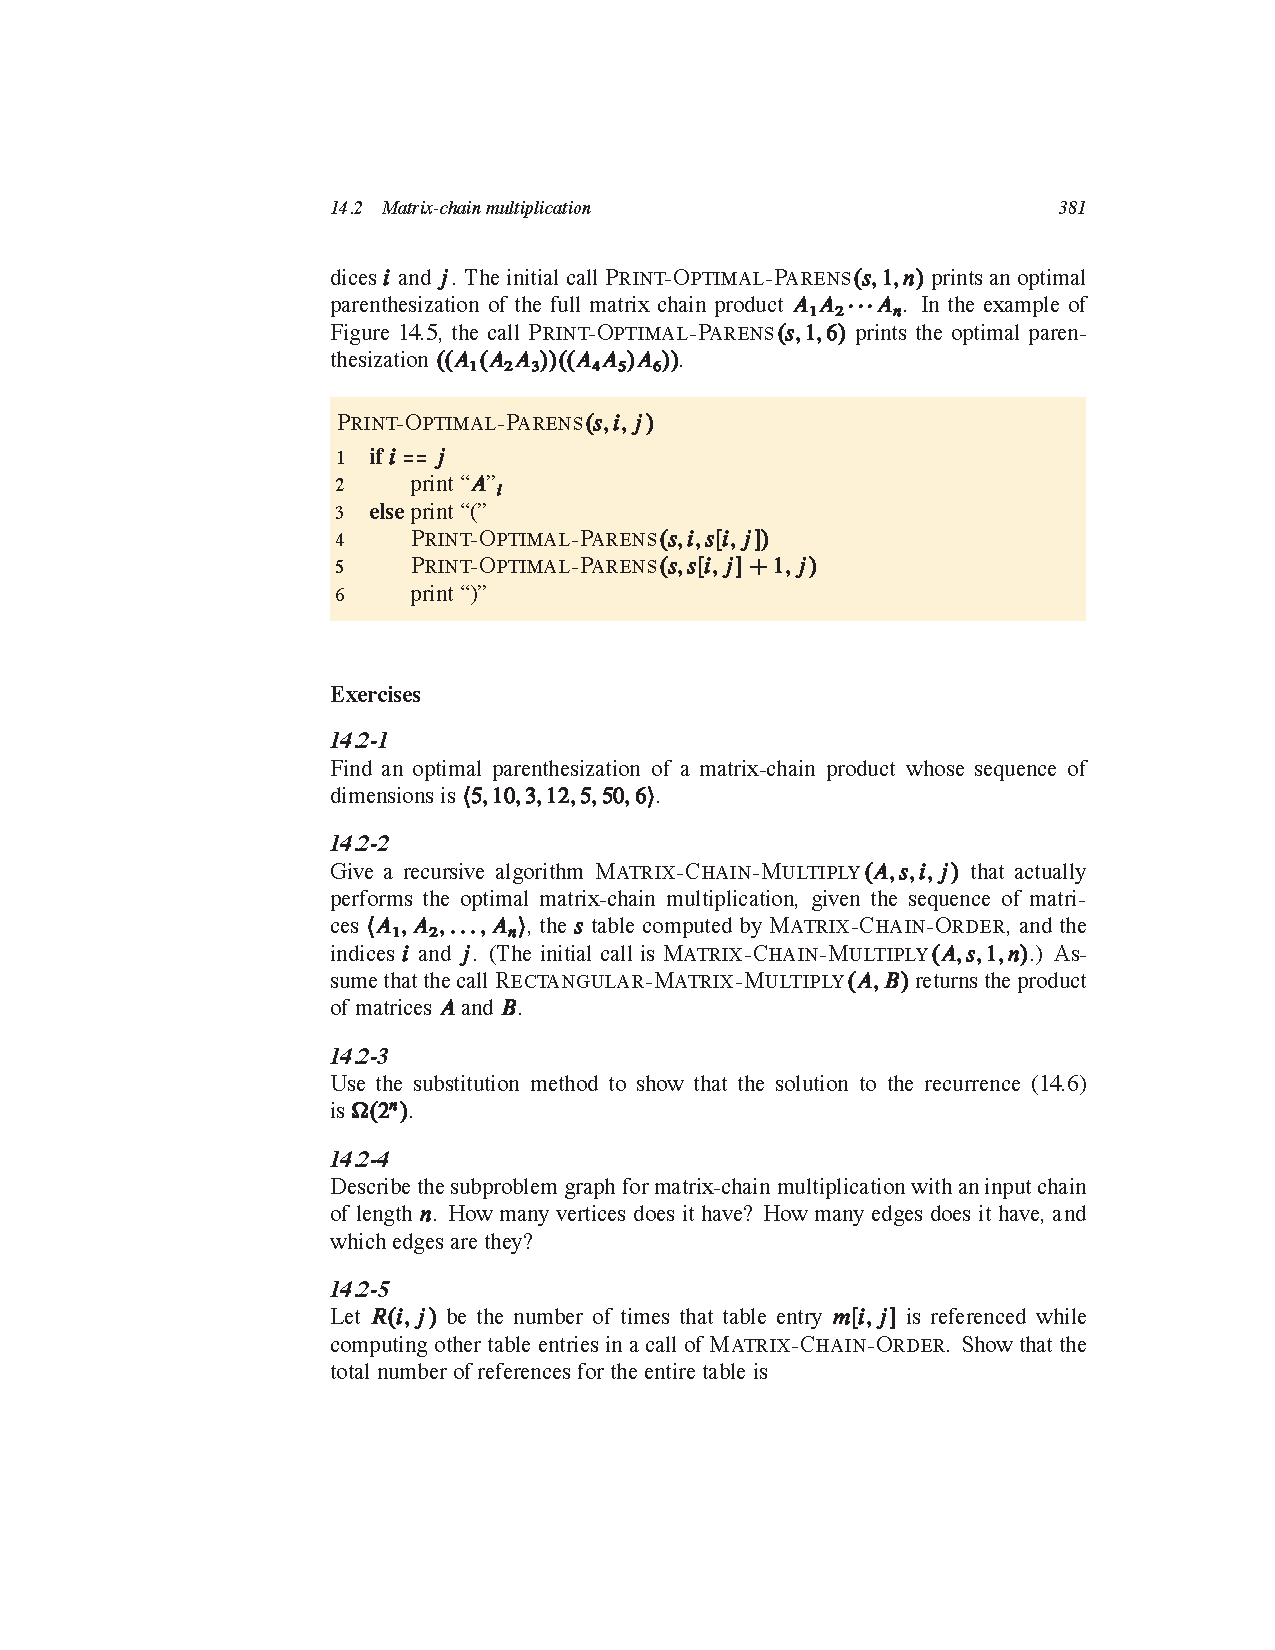
\includegraphics[width=\textwidth, trim={4cm 17cm 3cm 6.75cm}, clip]{figures/p381}
\end{frame}

\section{Optimal binary search trees}

\begin{frame}{Optimal binary search trees}
    \begin{itemize}
        \item Given sequence $K = \langle k_1, k_2, \ldots, k_n \rangle$ of $n$ distinct keys, sorted $(k_1 < k_2 < \ldots < k_n)$.
        \item Want to build a binary search tree from the keys.
        \item For $k_i$, have probability $p_i$ that a search is for $k_i$.
        \item Want BST with minimum expected search cost.
    \end{itemize}
\end{frame}

\begin{frame}{BST Cost}
    Actual cost = \# of items examined.
    \begin{center}
        \footnotesize
        For $k_i$, $cost = depth_T (k_i) + 1$, where $depth_T (k_i) =$ depth $k_i$ in BST $T$.
    \end{center}
    $E[$ search cost in $T]$
    \begin{equation*}
        \begin{align*}
            =& \sum_{i=n}^{n} (depth_T(k_i) + 1) \cdot p_i \\
            =& \sum_{i=n}^{n} depth_T(k_i) \cdot p_i + \sum_{i=1}^{n} p_i \\
            =& 1 + \sum_{i=n}^{n} depth_T(k_i) \cdot p_i
        \end{align*}
    \end{equation*}
\end{frame}

\begin{frame}{Example}
    \centering
    \begin{tabular}{c | c c c c c}
        i & 1 & 2 & 3 & 4 & 5 \\
        \hline
        $p_i$ & .25 & .2 & .05 & .2 & .3
    \end{tabular}
    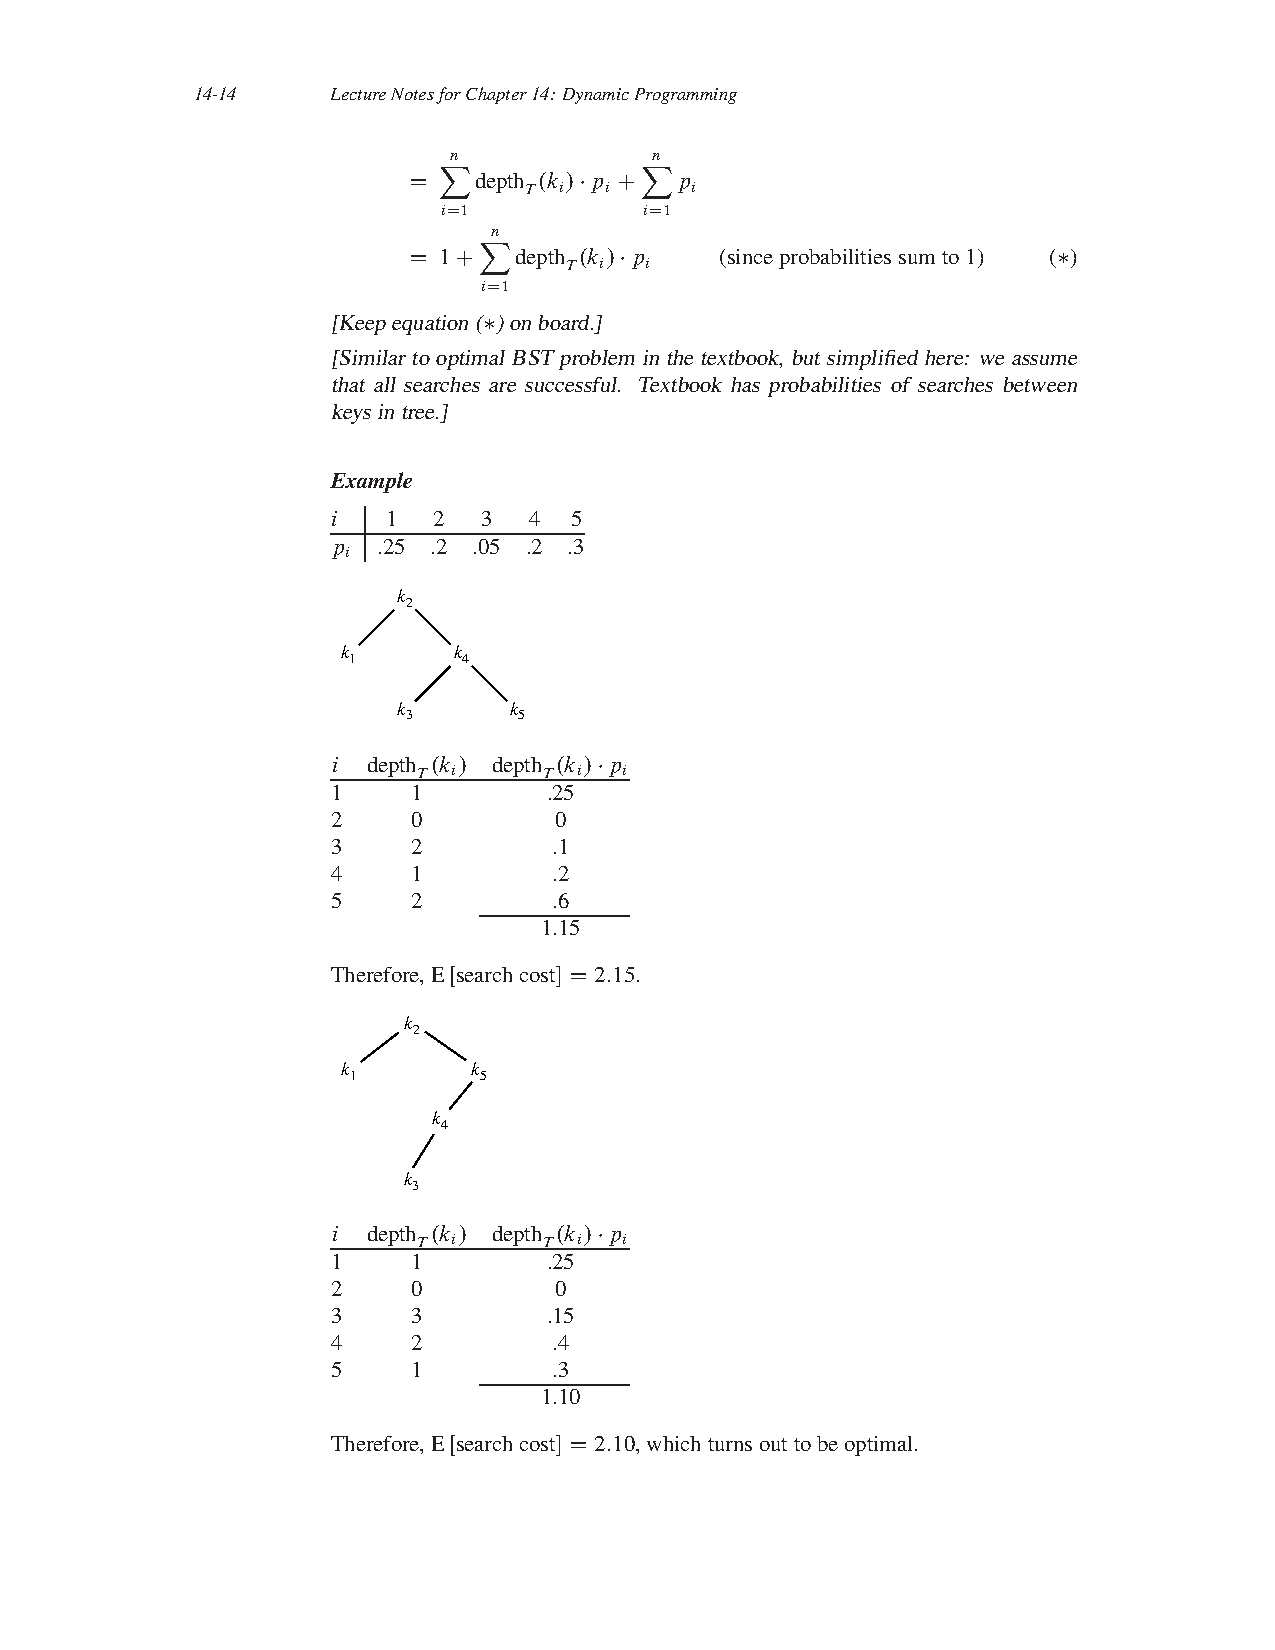
\includegraphics[width=\textwidth, trim={4cm 12cm 4cm 9.75cm}, clip]{figures/BST_example}
    \begin{itemize}
        \item Therefore, E[search cost] = 2.15.
    \end{itemize}
\end{frame}

\begin{frame}{Example}
    \centering
    \begin{tabular}{c | c c c c c}
        i & 1 & 2 & 3 & 4 & 5 \\
        \hline
        $p_i$ & .25 & .2 & .05 & .2 & .3
    \end{tabular}
    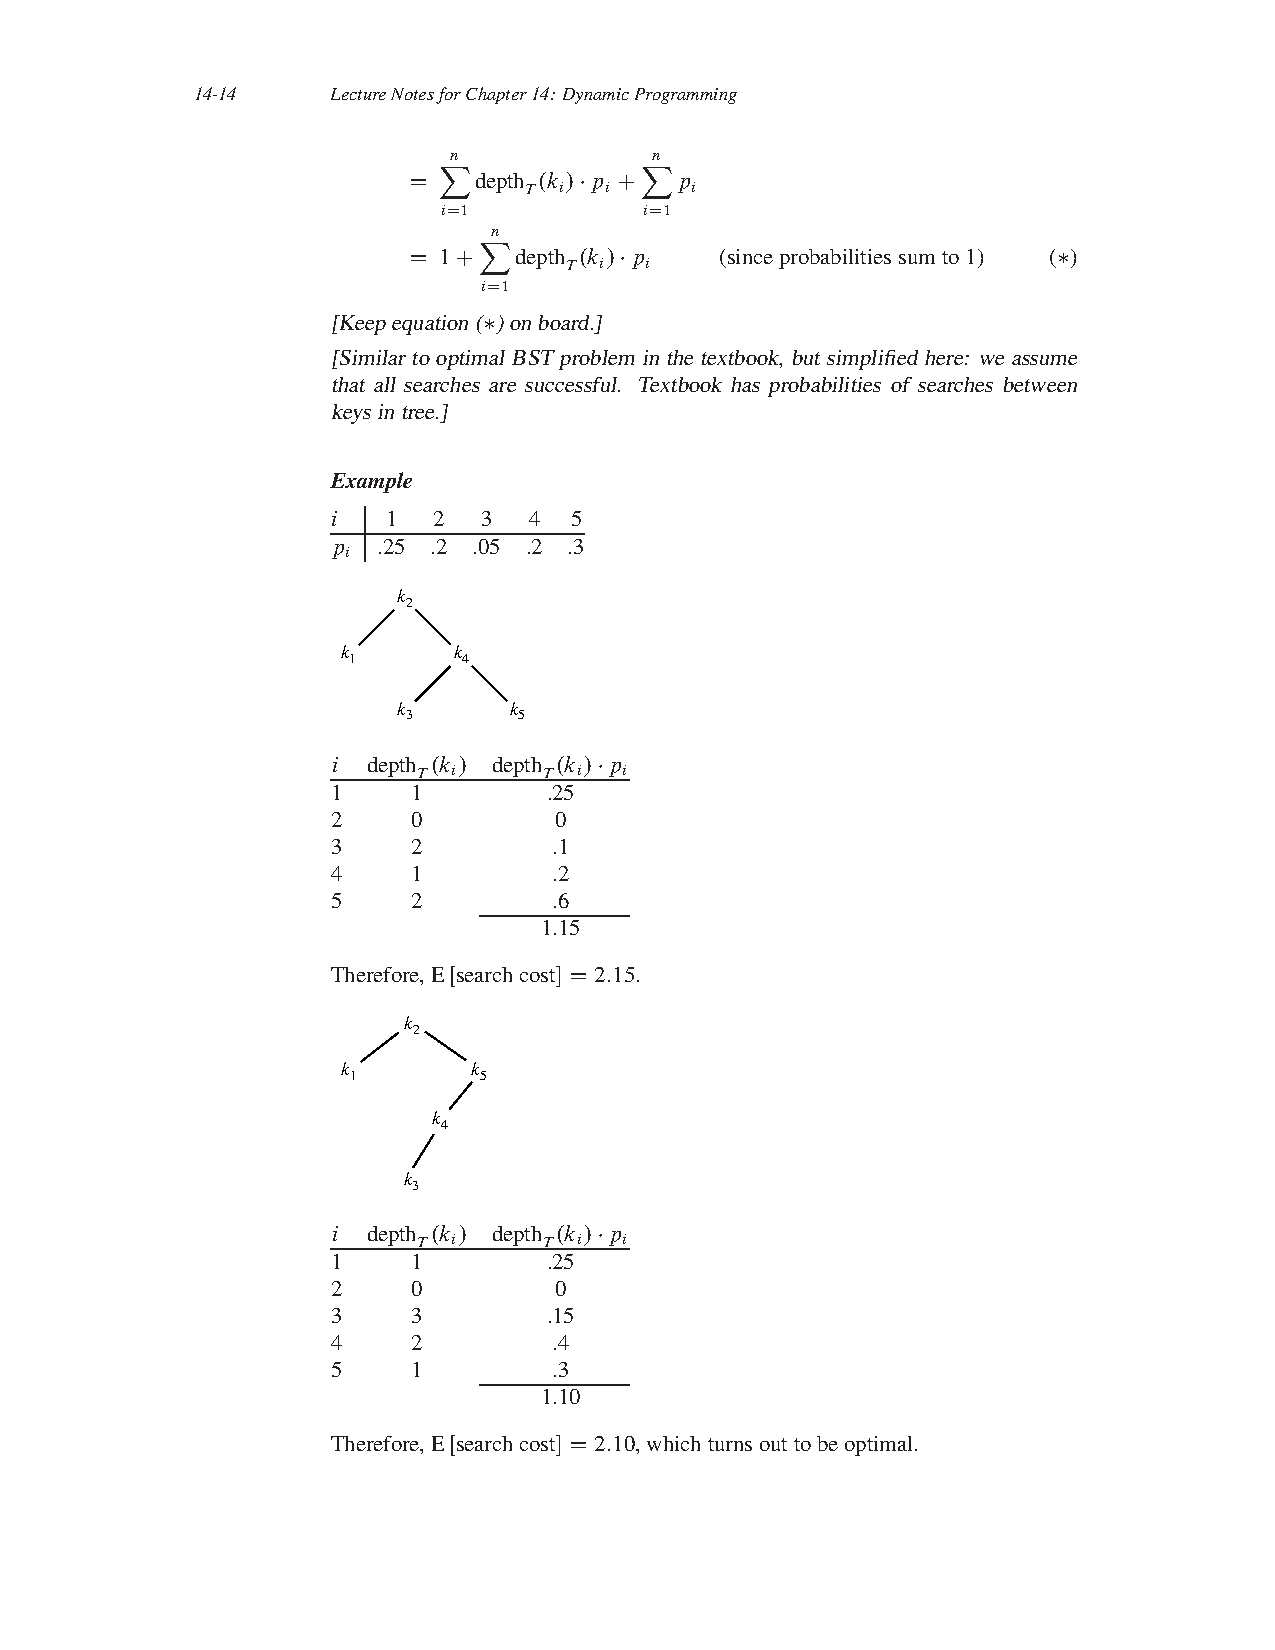
\includegraphics[width=\textwidth, trim={4cm 4cm 4cm 17cm}, clip]{figures/BST_example}
    \begin{itemize}
        \item Therefore, E[search cost] = 2.10, which turns out to be optimal.
    \end{itemize}
\end{frame}

\begin{frame}{Observations}
    \begin{itemize}
        \item Optimal BST might not have smallest height.
        \item Optimal BST might not have highest-probability key at root.
    \end{itemize}
    Build by exhaustive checking?
    \begin{itemize}
        \item Construct each $n$-node BST.
        \item For each, put in keys.
        \item Then compute expected search cost.
        \item But there are $\Omega \left( \frac{4^n}{n^{\frac{3}{2}}} \right)$ different BSTs with $n$ nodes.
    \end{itemize}
\end{frame}

\begin{frame}{Step 1: The structure of an optimal BST}
    Consider any subtree of a BST.  It contains keys in a contiguous range $k_i, \ldots, k_j$ for some $1 \leq i \leq j \leq n$.

    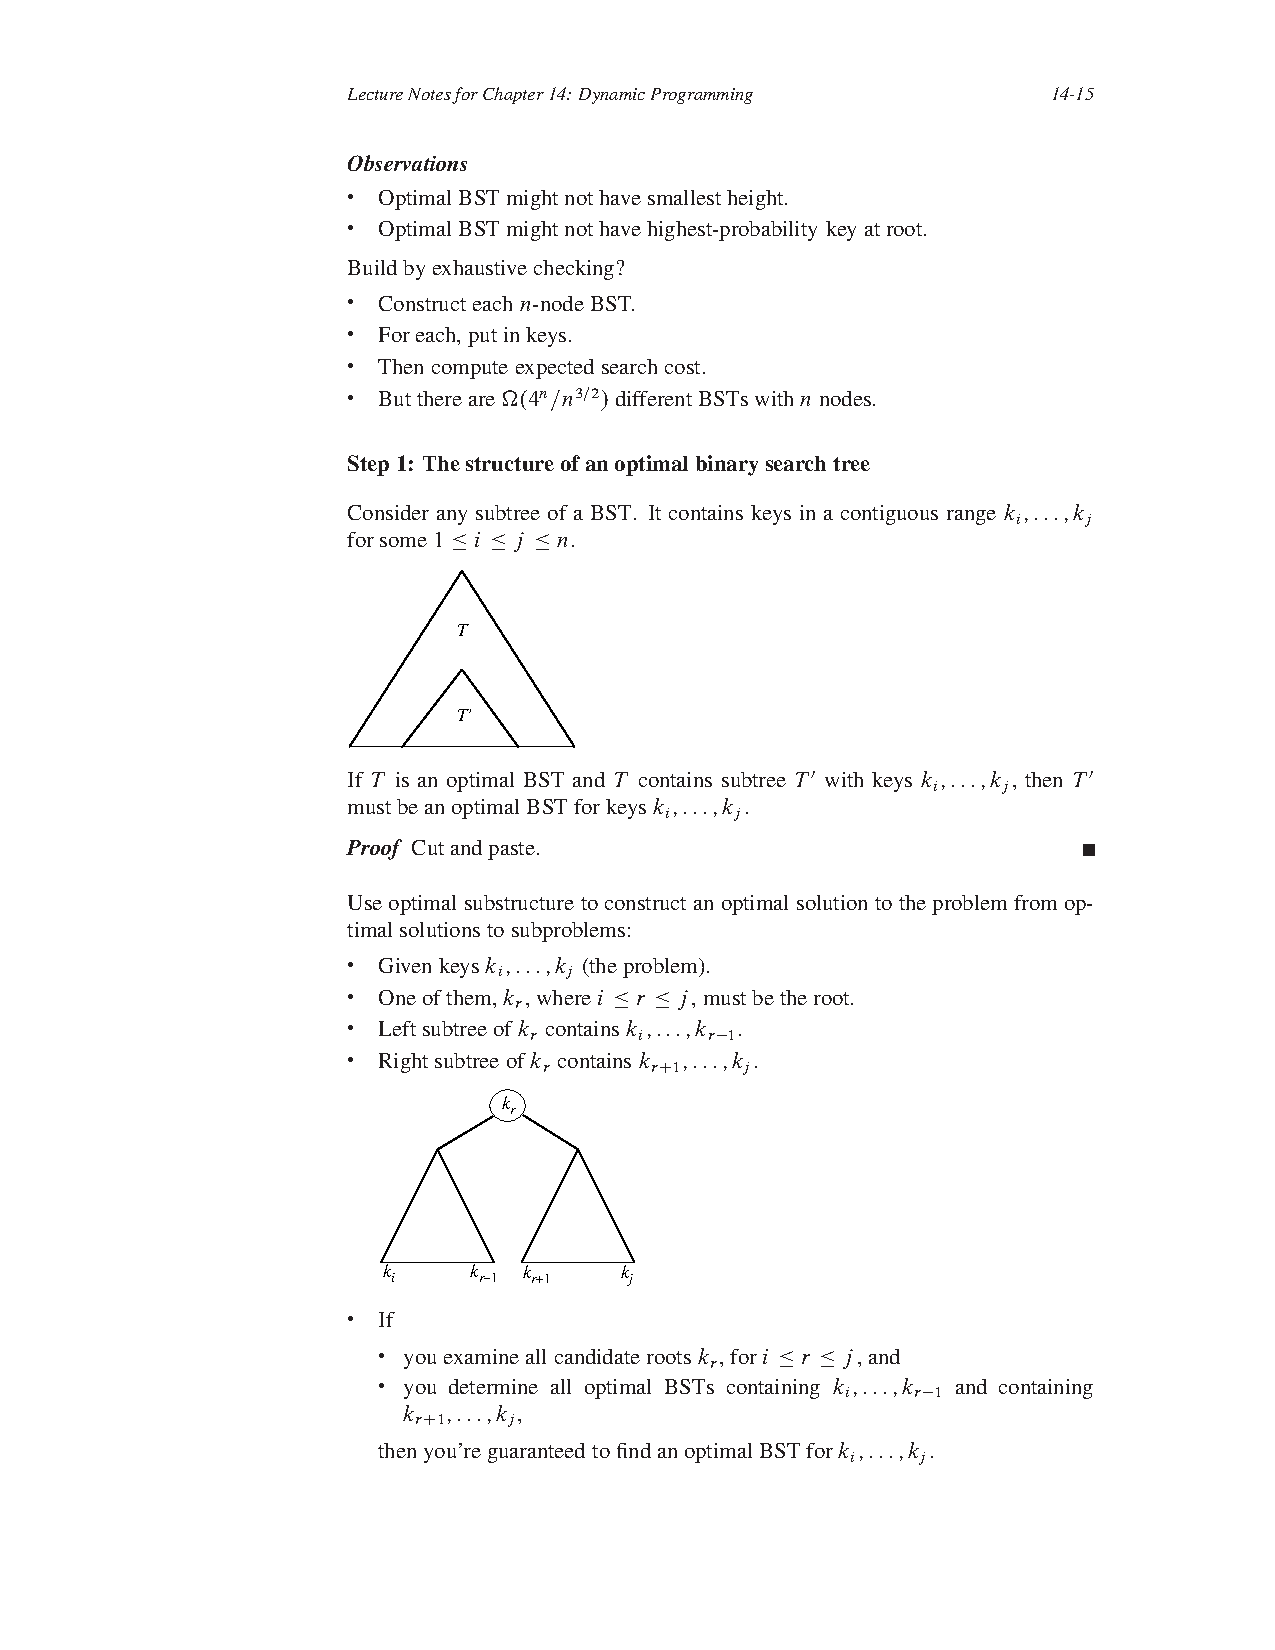
\includegraphics[width=\textwidth, trim={4cm 15cm 4cm 9.5cm}, clip]{figures/BST_step1}

    If $T$ is an optimal BST and $T$ contains subtree $T^\prime$ with keys $k_i, \ldots, k_j$, then $T^\prime$ must be an optimal BST for keys $k_i, \ldots, k_j$.
\end{frame}

\begin{frame}{Step 1: The structure of an optimal BST}
    Use optimal substructure to construct an optimal solution to the problem from optimal solutions to subproblems:
    \begin{itemize}
        \item Given keys $k_i, \ldots, k_j$ (the problem).
        \item One of them, $k_r$, where $i \leq r \leq j$, must be the root.
        \item Left subtree of $k_r$ contains $k_i, \ldots, k_{r-1}$.
        \item Right subtree of $k_r$ contains $k_{r+1}, \dots, k_j$.
    \end{itemize}
    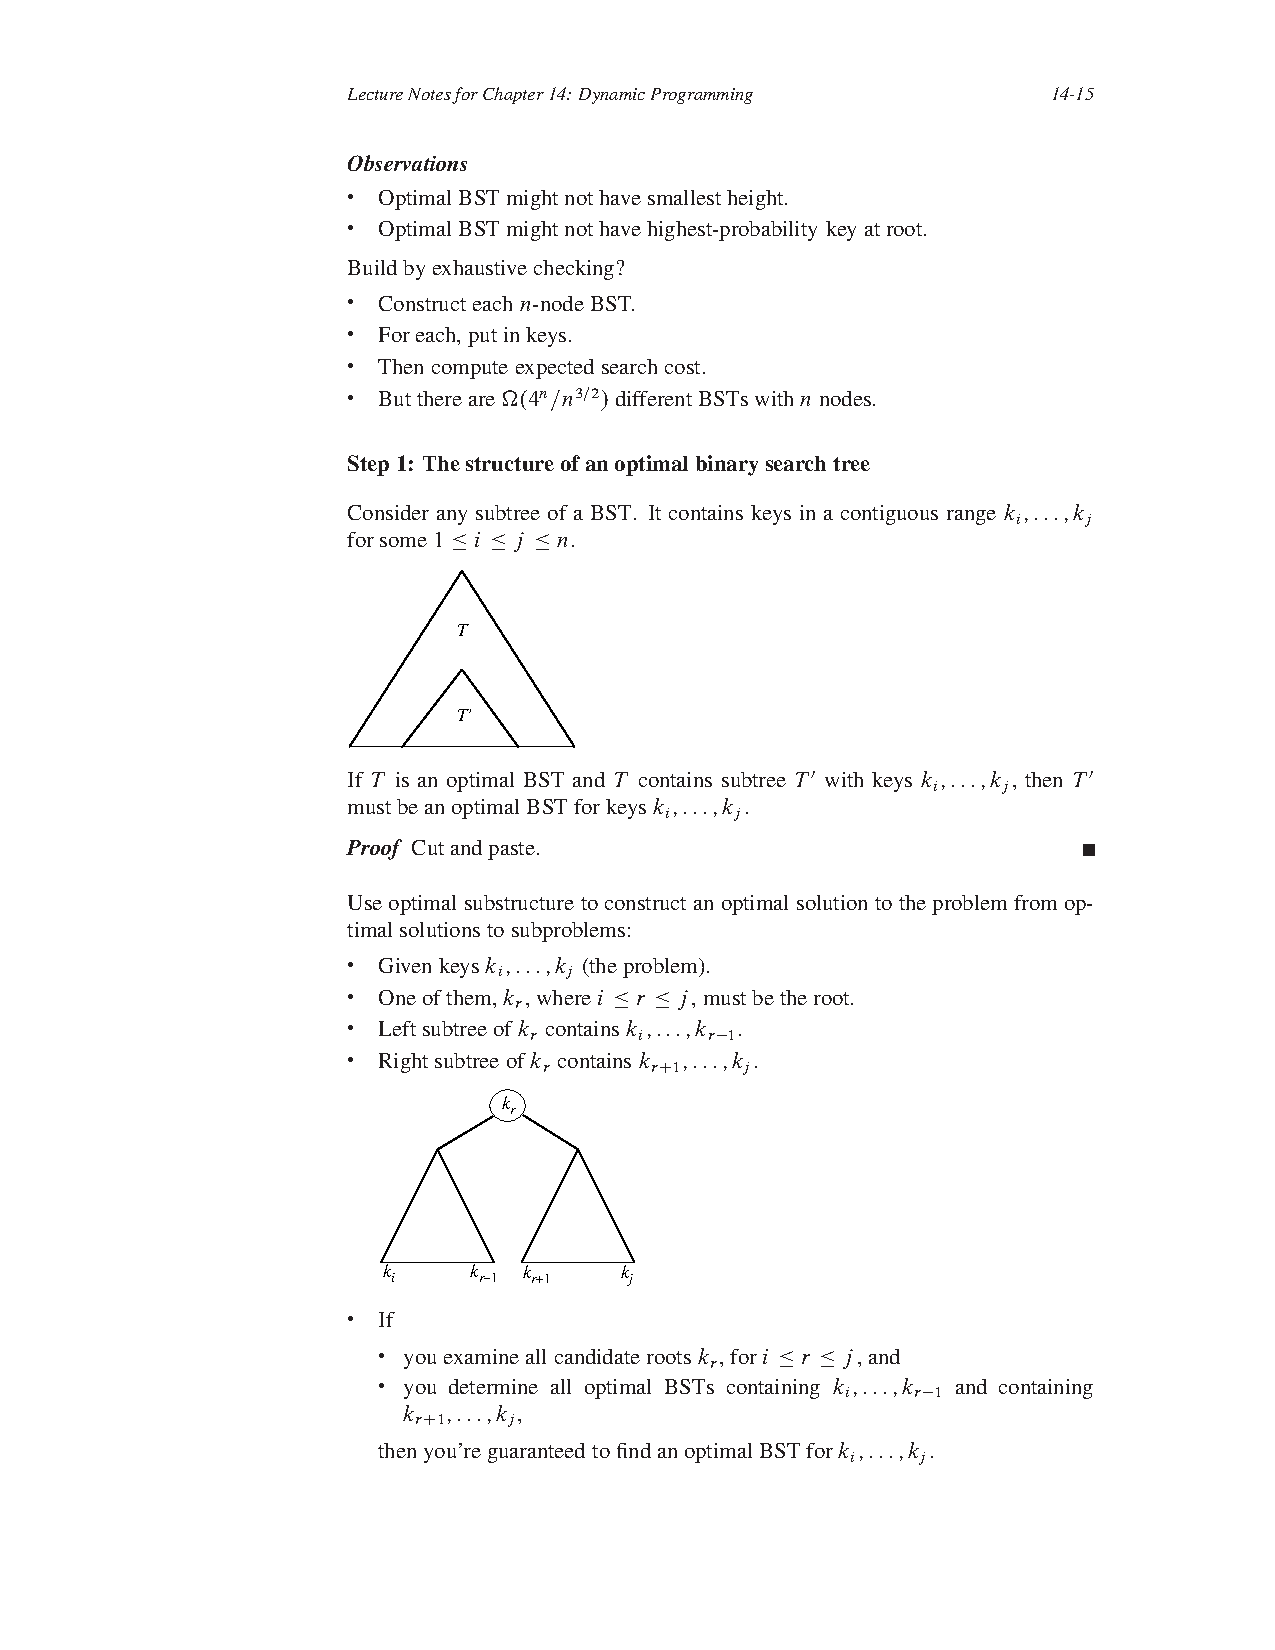
\includegraphics[width=\textwidth, trim={4cm 6cm 4cm 18.25cm}, clip]{figures/BST_step1}
\end{frame}

\begin{frame}{Step 1: The structure of an optimal BST}
    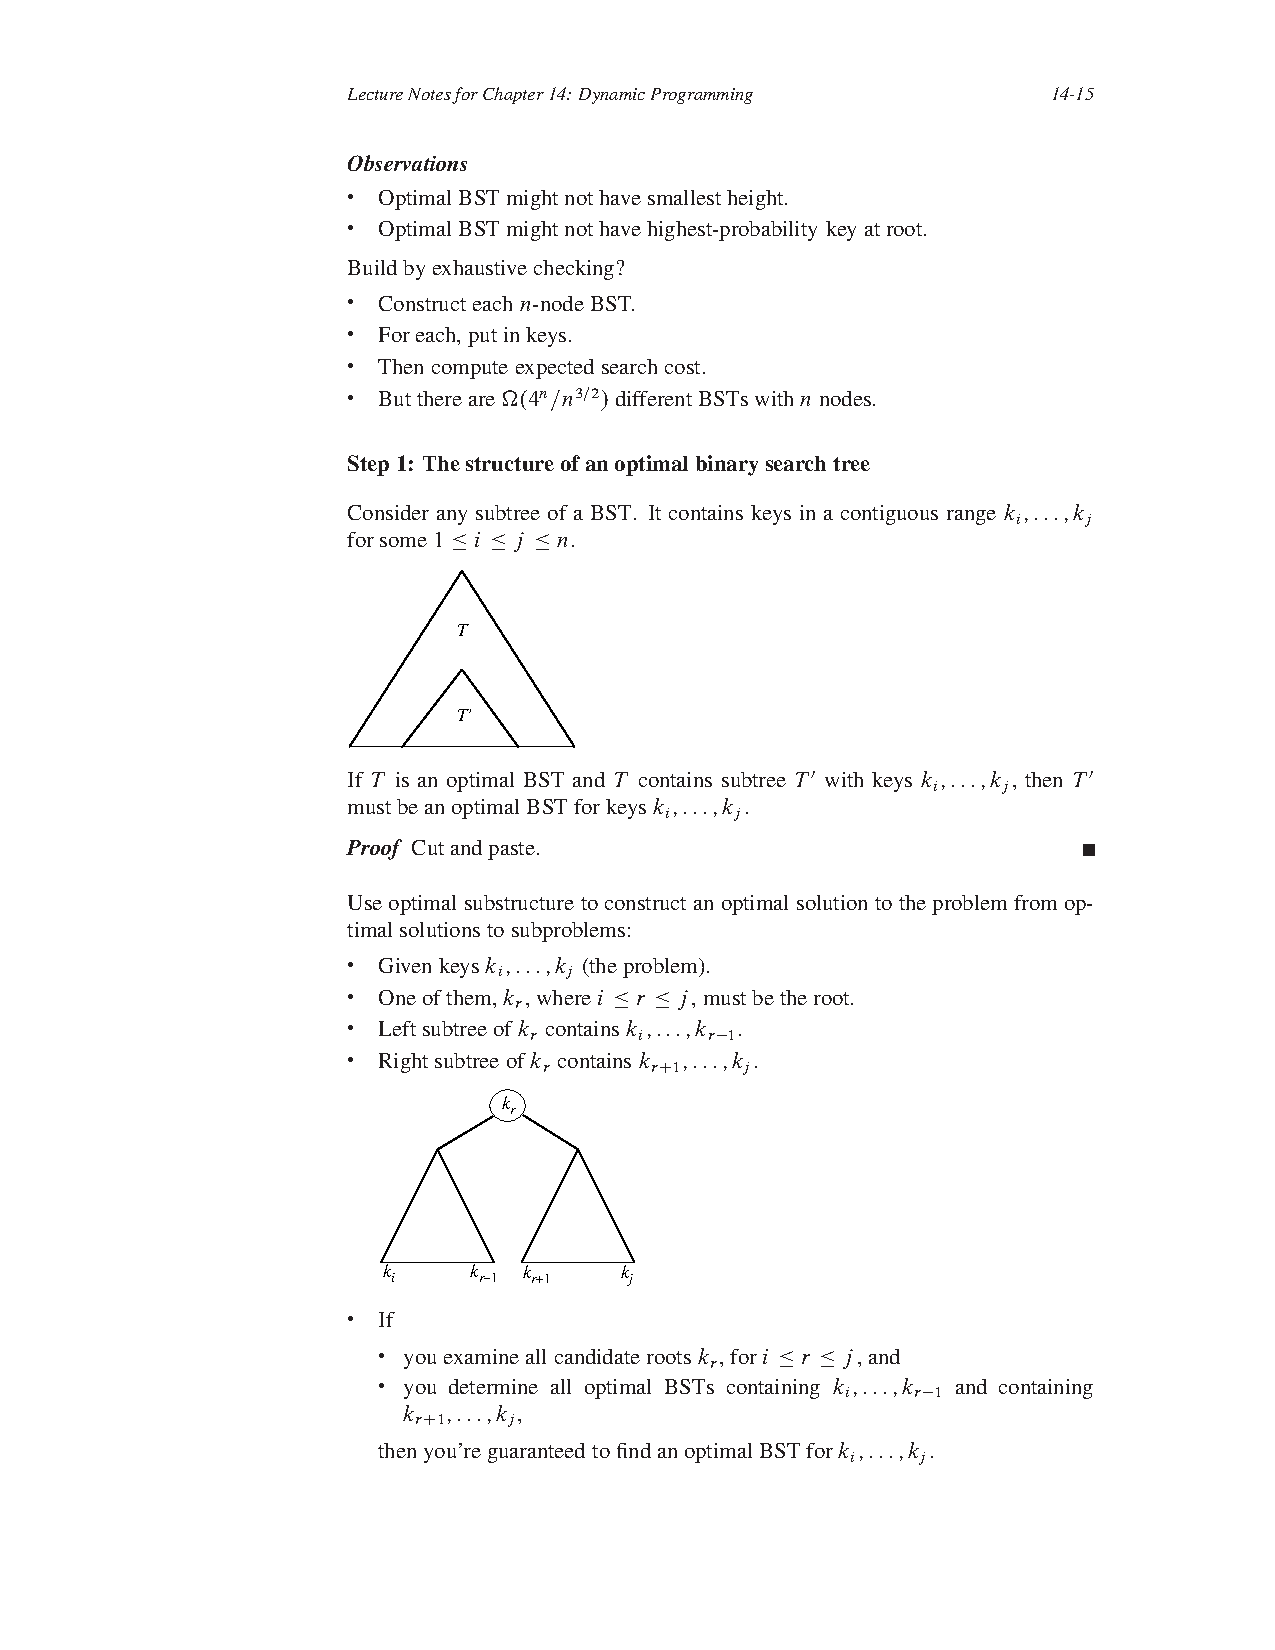
\includegraphics[width=\textwidth, trim={4cm 6cm 4cm 18.25cm}, clip]{figures/BST_step1}
    \begin{itemize}
        \item If
            \begin{itemize}
                \item you examine all candidate roots $k_r$, for $i \leq r \leq j$, and
                \item you determine all optimal BSTs containing $k_i, \ldots, k_{r-1}$ and containing $k_{r+1}, \ldots, k_j$,
            \end{itemize}
        then you're guaranteed to find an optimal BST for $k_i, \ldots, k_j$.
    \end{itemize}
\end{frame}

\begin{frame}{Step 2: Recursive solution}
    Subproblem domain:
    \begin{itemize}
        \item Find optimal BST for $k_i, \ldots, k_j$, where $i \geq 1$, $j \leq n$, $j \geq i - 1$.
        \item When $j = i - 1$, the tree is empty.
    \end{itemize}
    Define $e[i, j] = $ expected search cost of optimal BST for $k_i, \dots, k_j$.
\end{frame}

\begin{frame}{Step 2: Recursive solution}
    \begin{itemize}
        \item If $j = i - 1$, then $e[i, j] = 0$.
        \item If $j \geq i$,
            \begin{itemize}
                \item Select root $k_r$, for some $i \leq r \leq j$.
                \item Make an optimal BST with $k_i, \ldots, k_{r-1}$ as the left subtree.
                \item Make an optimal BST with $k_{r+1}, \ldots, k_j$ as the right subtree.
                \item Note: when $r = i$, left subtree is $k_i, \dots, k_{i-1}$; when $r = j$, right subtree is $k_{j+1}, \ldots, k_j$.  These subtrees are empty.
            \end{itemize}
    \end{itemize}
\end{frame}

\begin{frame}{Step 2: Recursive solution}
    When a subtree becomes a subtree of a node:
    \begin{itemize}
        \item Depth of every node in subtree goes up by 1.
        \item Expected search cost increases by
            \begin{equation*}
                \begin{align*}
                    w(i, j) = \sum_{l = i}^{j} p_l
                \end{align*}
            \end{equation*}
    \end{itemize}
    If $k_r$ is the root of an optimal BST for $k_i, \ldots, k_j$:
        \begin{equation*}
            \begin{align*}
                e[i, j] = p_r + (e[i, r-1] + w(i, r-1)) + (e[r+1, j] + w(r+1, j))
            \end{align*}
        \end{equation*}
    \begin{itemize}
        \item But $w(i, j) = w(i, r-1) + p_r + w(r+1, j)$.
        \item Therefore, $e[i, j] = e[i,r-1] + e[r+1, j] + w(i, j)$
    \end{itemize}
\end{frame}

\begin{frame}{Step 2: Recursive solution}
    That equation assumes that we already know which key is $k_r$.  We don’t.
    \begin{itemize}
        \item Try all candidates, and pick the best one:
            \begin{equation*}
                \scriptsize
                \begin{align*}
                    e[i, j] =
                        \begin{cases}
                            0 & \text{ if } j = i - 1 \text{,} \\
                            \min \left \{ e[i, r-1] + e[r+1, j] + w(i, j):i \leq r \leq j \right \} & \text{ if } i \leq j \text{.}
                        \end{cases}
                \end{align*}
            \end{equation*}
        \item Could write a recursive algorithm. . .
    \end{itemize}
\end{frame}

\begin{frame}{}
\end{frame}
% \begin{frame}{}
%    \begin{minted}
%    [tabsize=4, obeytabs, frame=lines, framesep=2mm, baselinestretch=1.2, bgcolor=LightGray, fontsize=\scriptsize]{sql}
%    \end{minted}
% \end{frame}

%     \begin{codebox}
%         \Procname{$\proc{Insertion-Sort}(A)$}
%         \li \For $j \gets 2$ \To $\id{length}[A]$
%         \li \Do
%         $\id{key} \gets A[j]$
%         \li \Comment Insert $A[j]$ into the sorted sequence
%         $A[1 \twodots j-1]$.
%         \li $i \gets j-1$
%         \li \While $i > 0$ and $A[i] > \id{key}$
%         \li \Do
%         $A[i+1] \gets A[i]$
%         \li $i \gets i-1$
%         \End
%         \li $A[i+1] \gets \id{key}$
%         \End
%     \end{codebox}

\begin{frame}{Introduction to Algorithms}
    \centering
    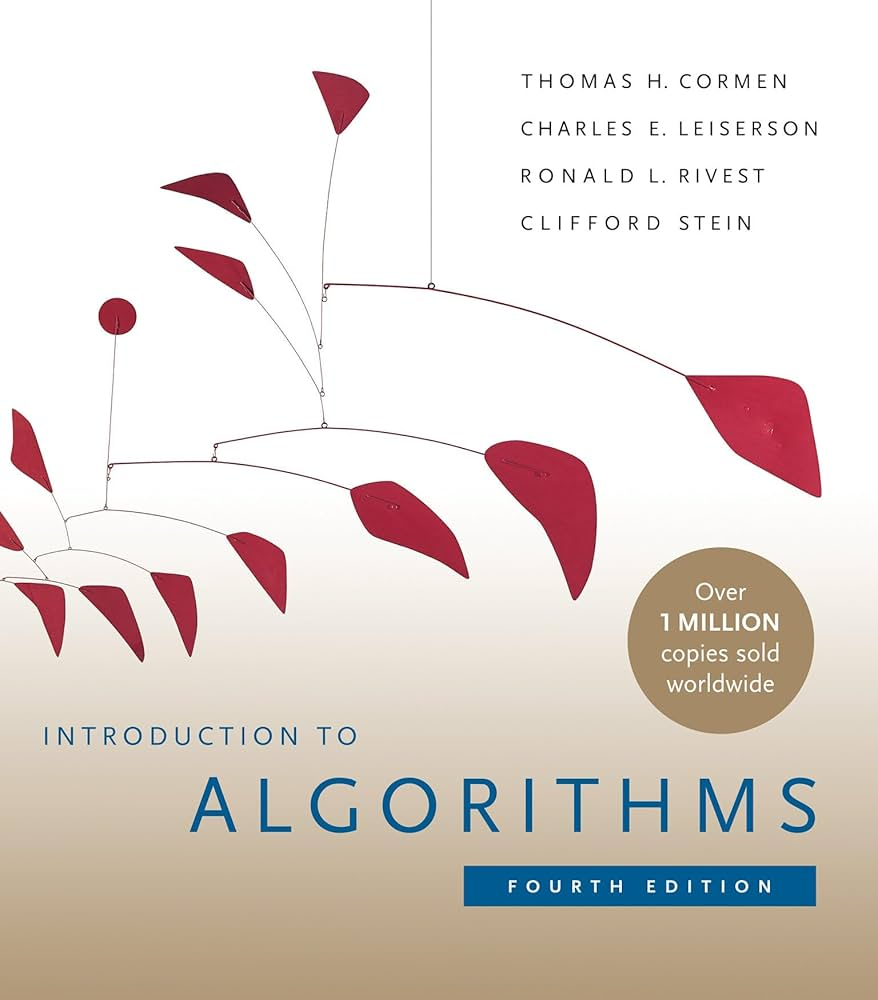
\includegraphics[width=0.45\textwidth]{figures/book_cover.jpg} \\
    \vspace{5mm}{
        \tiny
        Content has been extracted from \textit{Introduction to Algorithms}, Fourth Edition, by Cormen, Leiserson, Rivest, and Stein. MIT Press. 2022.\\
        Visit \url{https://mitpress.mit.edu/9780262046305/introduction-to-algorithms/}.
    }
\end{frame}

\end{document}
